\subsection{Effect of Communication Networks on  Trajectories}\label{apdx:communication_effect}

\begin{figure}[h]
    \centering
    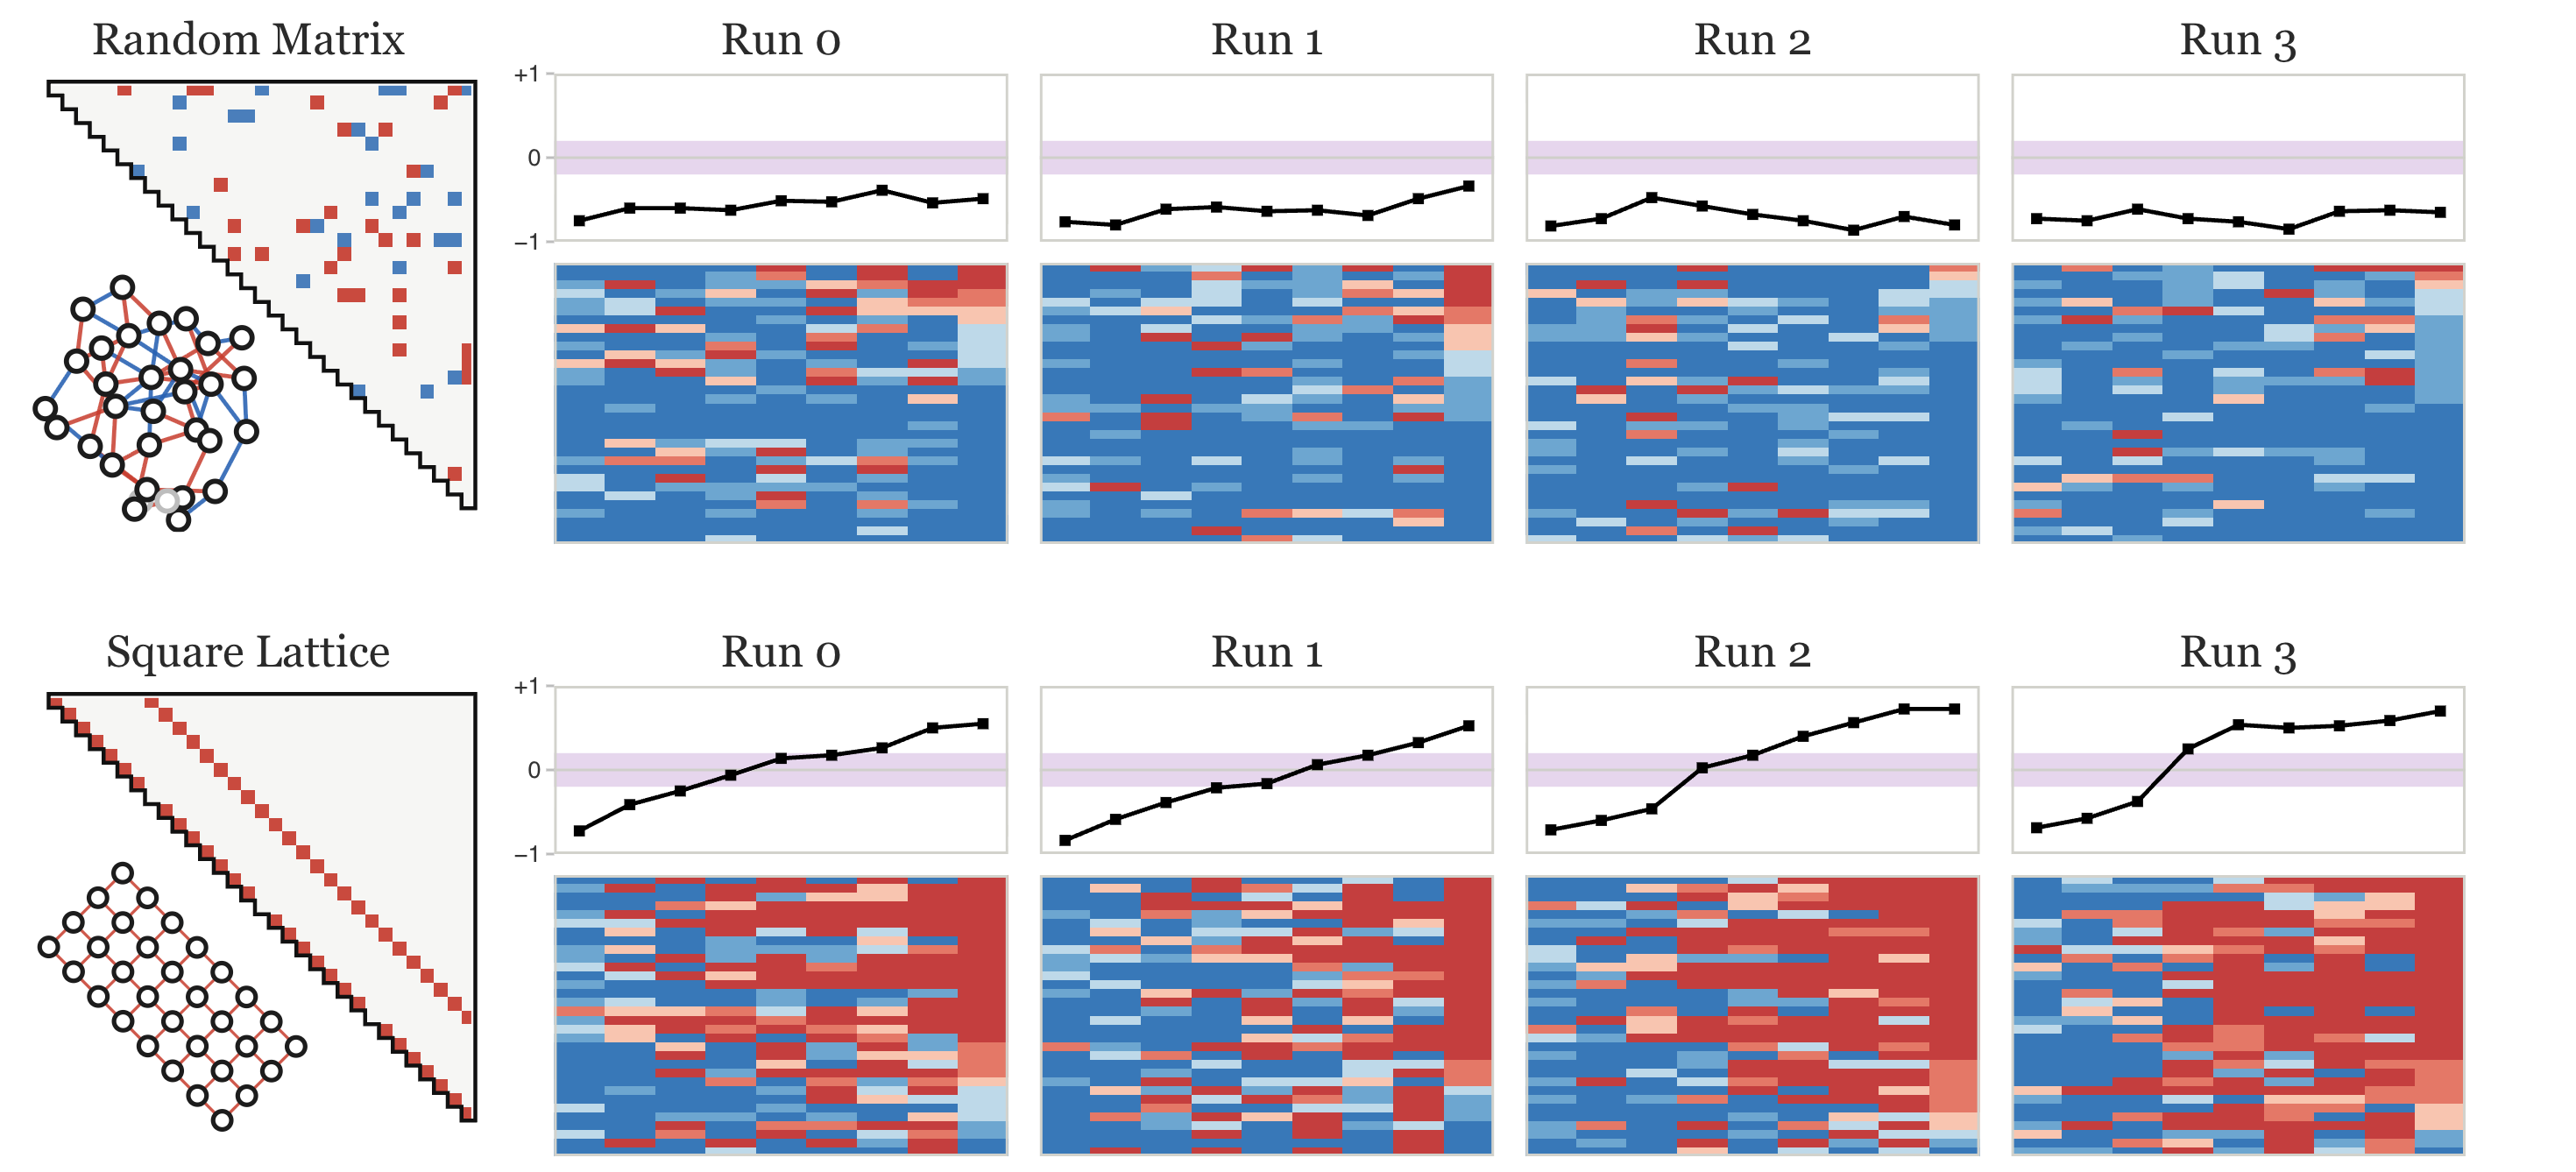
\includegraphics[width=0.99\textwidth]{main/Figures/apx_07_communication_networks.png}
\caption{\textit{Different communication networks can cause differences in trajectories.} Four episodes (labeled as runs 0-3) on the same question under two different social graphs: a random matrix (\emph{top}) and a square lattice (\emph{bottom}). For each graph, the left panel shows the couplings $J$ as a heatmap in the upper triangle and as a node-link diagram below it, and each of the four runs shows the net opinion $n(t)$ over rounds (\emph{line plot at the top}) together with the group trajectory (\emph{heatmap at the bottom}). Under the random matrix the community stays on its initial side across all four runs, while under the square lattice it crosses the split band and settles on the opposite side in all four runs. This is not a common situation, but social graphs can cause consistent differences between how group trajectories evolve when answering the same question. In other words, the social connections carry information about where will the community end up, even before any messages are exchanged.}
\label{fig:communication_networks}
\end{figure}
